%%%%%%%%%%%%%%%%%%%%%%%%%%%%%%%%%%%%%%%%%
% Beamer Presentation
% LaTeX Template
% Version 1.0 (10/11/12)
%
% This template has been downloaded from:
% http://www.LaTeXTemplates.com
%
% License:
% CC BY-NC-SA 3.0 (http://creativecommons.org/licenses/by-nc-sa/3.0/)
%
%%%%%%%%%%%%%%%%%%%%%%%%%%%%%%%%%%%%%%%%%

%----------------------------------------------------------------------------------------
%	PACKAGES AND THEMES
%----------------------------------------------------------------------------------------

\documentclass{beamer}

\mode<presentation> {

% The Beamer class comes with a number of default slide themes
% which change the colors and layouts of slides. Below this is a list
% of all the themes, uncomment each in turn to see what they look like.

%\usetheme{default}
%\usetheme{AnnArbor}
%\usetheme{Antibes}
%\usetheme{Bergen}
%\usetheme{Berkeley}
%\usetheme{Berlin}
%\usetheme{Boadilla}
%\usetheme{CambridgeUS}
%\usetheme{Copenhagen}
%\usetheme{Darmstadt}
%\usetheme{Dresden}
%\usetheme{Frankfurt}
%\usetheme{Goettingen}
%\usetheme{Hannover}
%\usetheme{Ilmenau}
%\usetheme{JuanLesPins}
%\usetheme{Luebeck}
\usetheme{Madrid}
%\usetheme{Malmoe}
%\usetheme{Marburg}
%\usetheme{Montpellier}
%\usetheme{PaloAlto}
%\usetheme{Pittsburgh}
%\usetheme{Rochester}
%\usetheme{Singapore}
%\usetheme{Szeged}
%\usetheme{Warsaw}

% As well as themes, the Beamer class has a number of color themes
% for any slide theme. Uncomment each of these in turn to see how it
% changes the colors of your current slide theme.

%\usecolortheme{albatross}
%\usecolortheme{beaver}
%\usecolortheme{beetle}
%\usecolortheme{crane}
%\usecolortheme{dolphin}
%\usecolortheme{dove}
%\usecolortheme{fly}
%\usecolortheme{lily}
%\usecolortheme{orchid}
%\usecolortheme{rose}
%\usecolortheme{seagull}
%\usecolortheme{seahorse}
%\usecolortheme{whale}
%\usecolortheme{wolverine}

%\setbeamertemplate{footline} % To remove the footer line in all slides uncomment this line
%\setbeamertemplate{footline}[page number] % To replace the footer line in all slides with a simple slide count uncomment this line

%\setbeamertemplate{navigation symbols}{} % To remove the navigation symbols from the bottom of all slides uncomment this line
}

\usepackage{marvosym}

%%% Работа с русским языком
\usepackage[T2A]{fontenc}			% кодировка
\usepackage[LGR,T1]{fontenc}
\usepackage[utf8]{inputenc}			% кодировка исходного текста
\usepackage[english, russian]{babel}	% локализация и переносы


\usepackage{graphicx} % Allows including images
\usepackage{booktabs} % Allows the use of \toprule, \midrule and \bottomrule in tables

\AtBeginSection[]
{
  \begin{frame}
    \frametitle{Содержание}
    \tableofcontents[currentsection]
  \end{frame}
}

%----------------------------------------------------------------------------------------
%	TITLE PAGE
%----------------------------------------------------------------------------------------

\title[Железный трон]{Дисперсионный анализ и Железный трон } % The short title appears at the bottom of every slide, the full title is only on the title page

\author{Борис Орехов} % Your name
\institute[НИУ ВШЭ] % Your institution as it will appear on the bottom of every slide, may be shorthand to save space
{
НИУ Высшая школа экономики \\ % Your institution for the title page
\medskip
\textit{nevmenandr@gmail.com} % Your email address
}
\date{5 июля 2016} % Date, can be changed to a custom date

\begin{document}

\begin{frame}
\titlepage % Print the title page as the first slide
\end{frame}

%------------------------------------------------

\begin{frame}
\begin{figure}
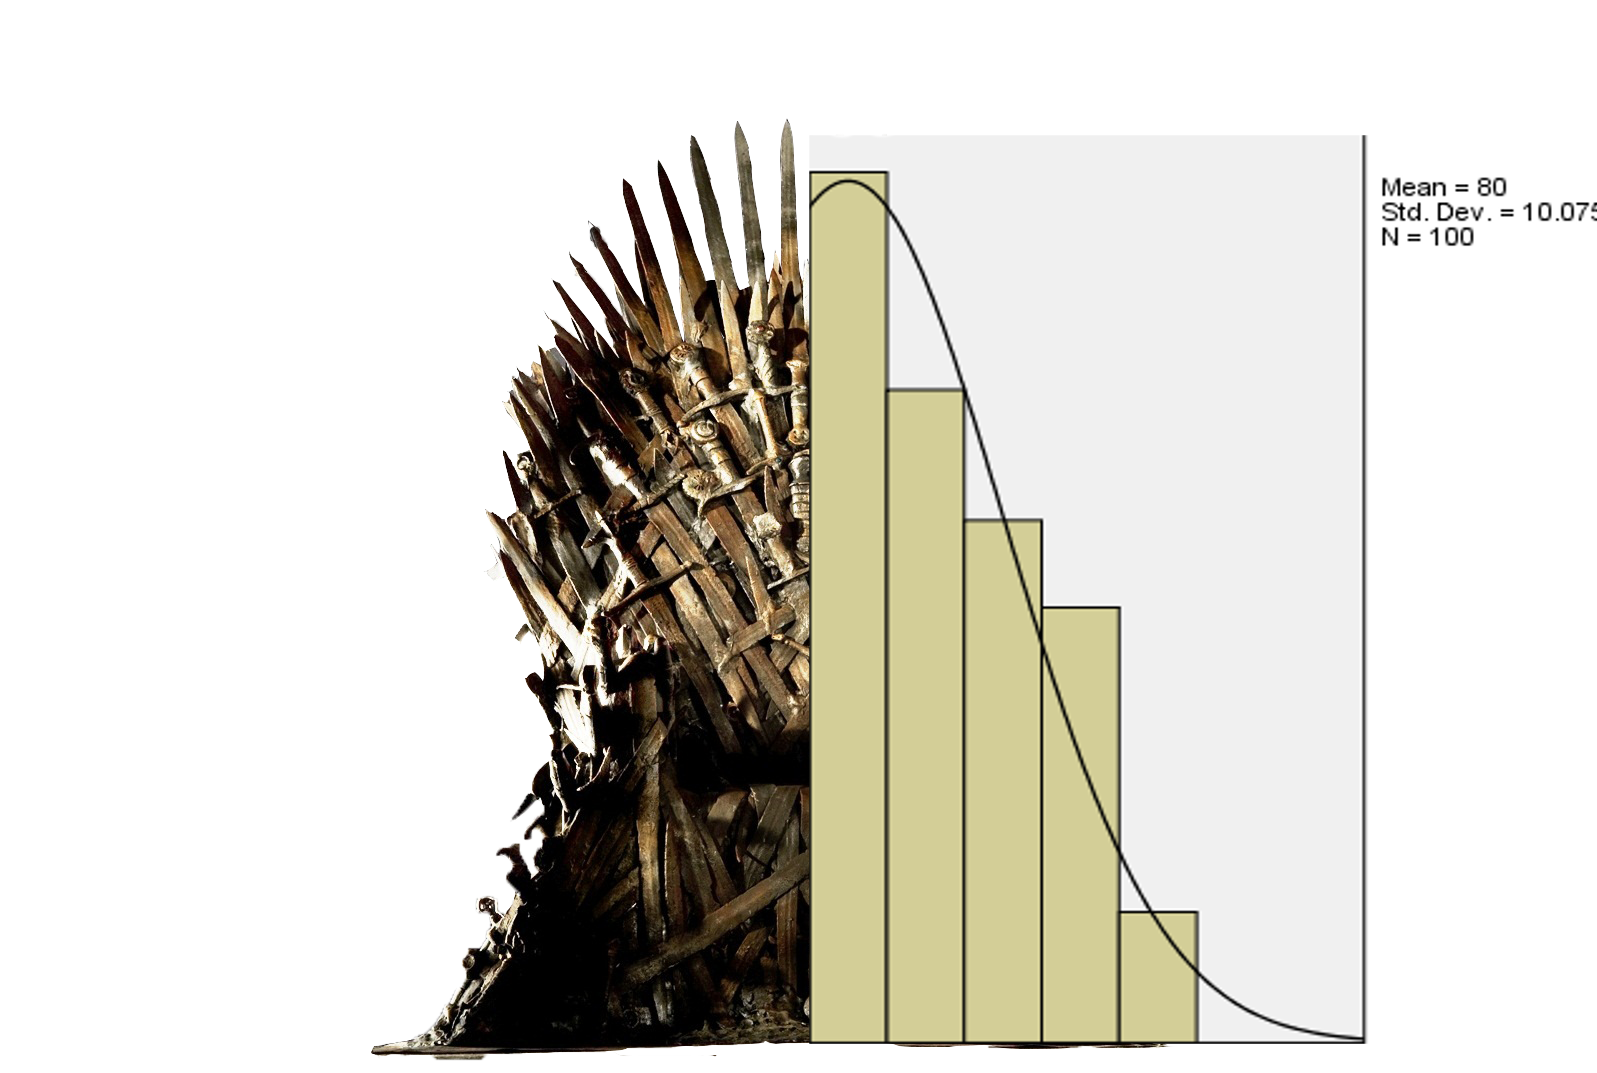
\includegraphics[width=0.9\linewidth]{iron_throne_data_analysis}
\end{figure}
\end{frame}

%------------------------------------------------

\begin{frame}
\frametitle{Содержание} % Table of contents slide, comment this block out to remove it
\tableofcontents % Throughout your presentation, if you choose to use \section{} and \subsection{} commands, these will automatically be printed on this slide as an overview of your presentation
\end{frame}

%----------------------------------------------------------------------------------------
%	PRESENTATION SLIDES
%----------------------------------------------------------------------------------------

%------------------------------------------------
\section{Вводные замечания} % Sections can be created in order to organize your presentation into discrete blocks, all sections and subsections are automatically printed in the table of contents as an overview of the talk
%------------------------------------------------

\subsection{Правда ли все дело в дисперсионном анализе?} % A subsection can be created just before a set of slides with a common theme to further break down your presentation into chunks



%------------------------------------------------

\begin{frame}
\frametitle{Дисперсионный анализ?}
Довольно много людей, записавшихся на~этот тьюториал (и~те, кто в~итоге сейчас здесь, и~те, кого мы~не~смогли пригласить), говорили, что~им интересно именно применение дисперсионного анализа к~художественному тексту.\\~\\

Должен признаться: упоминание именно дисперсионного анализа в~тексте "--- все"=таки рекламный трюк. На~самом деле речь будет идти об~анализе нарратива любым разумным статистическим способом. Если нам для~этого понадобятся графы или~векторные модели, которыми занимаются наши коллеги на~других тьюториалах, то нас это не~остановит.
\end{frame}

%------------------------------------------------

\subsection{Почему именно Дж. Мартин?}

\begin{frame}
\frametitle{Чем хороши книги Дж. Р. Р. Мартина?}
\begin{itemize}
\item Это \alert{большие} книги $\rightarrow$ большая выборка. Общий объем: 1.782.723 слова.
\item Цикл не~дописан и~(как в~естественных науках или~как с~идеями Соссюра о~реконструкции) можно будет получить независимое \alert{опровержение или~подтверждение} гипотезы, когда выйдут новые книги.
\item Благодаря сериалу книги \alert{популярны}, и~многие неплохо представляют, что~там происходит.
\end{itemize}
\end{frame}

\subsection{<<Игра престолов>> и статистика}

%------------------------------------------------

\begin{frame}
\frametitle{Статистика в Вестеросе}
\begin{block}{}
Люди обожают статистику. Вероятно, неполный список статистических этюдов об~<<Игре престолов>>:
\end{block}

\begin{itemize}
\item \cite{p1}
\item \cite{p9}
\item \cite{p2}
\item \cite{p7}
\item \cite{p8}
\item \cite{p3}
\end{itemize}

\begin{block}{}
Отдельно укажем аналитику с~использованием машинного обучения:
\end{block}

\cite{p4}, \cite{p5}, \cite{p11}

\end{frame}


\begin{frame}
\begin{figure}
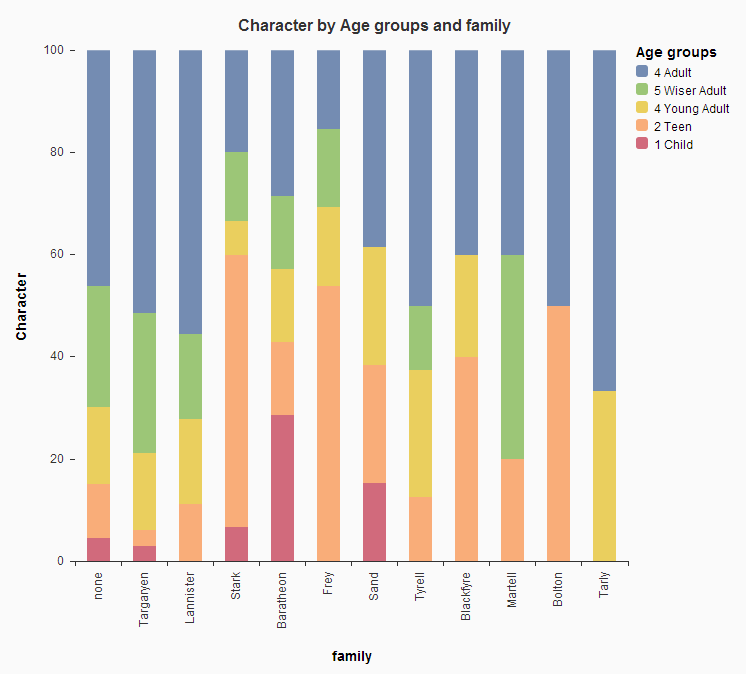
\includegraphics[width=0.7\linewidth]{diagr_age}
\end{figure}
\cite{p3}
\end{frame}

\begin{frame}
\begin{figure}
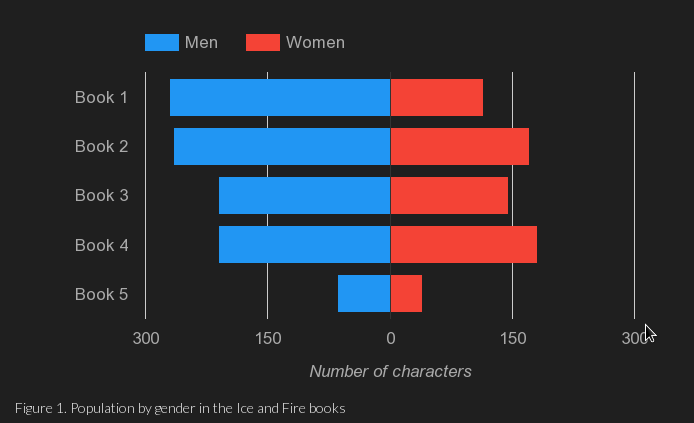
\includegraphics[width=0.9\linewidth]{IandF_gender}
\end{figure}
\cite{p1}
\end{frame}

\begin{frame}
Ср. данные из~другого источника:
\begin{figure}
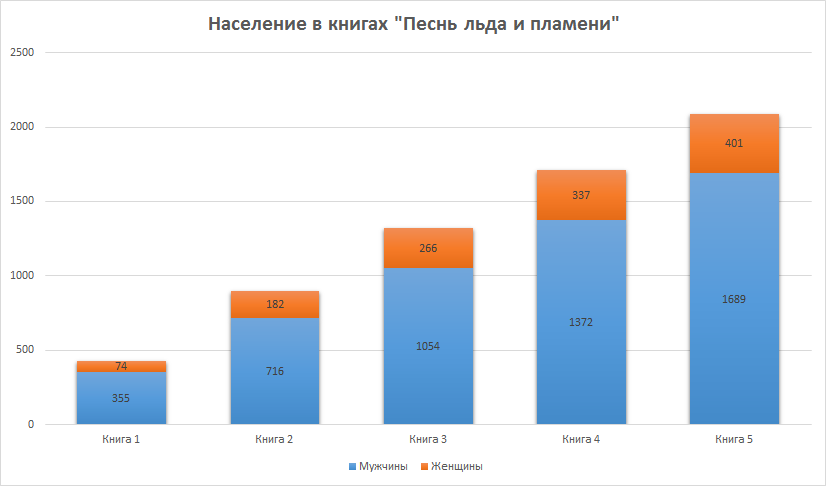
\includegraphics[width=0.8\linewidth]{IandF_gender2}
\end{figure}
\cite{p9}
\end{frame}

\begin{frame}
\begin{figure}
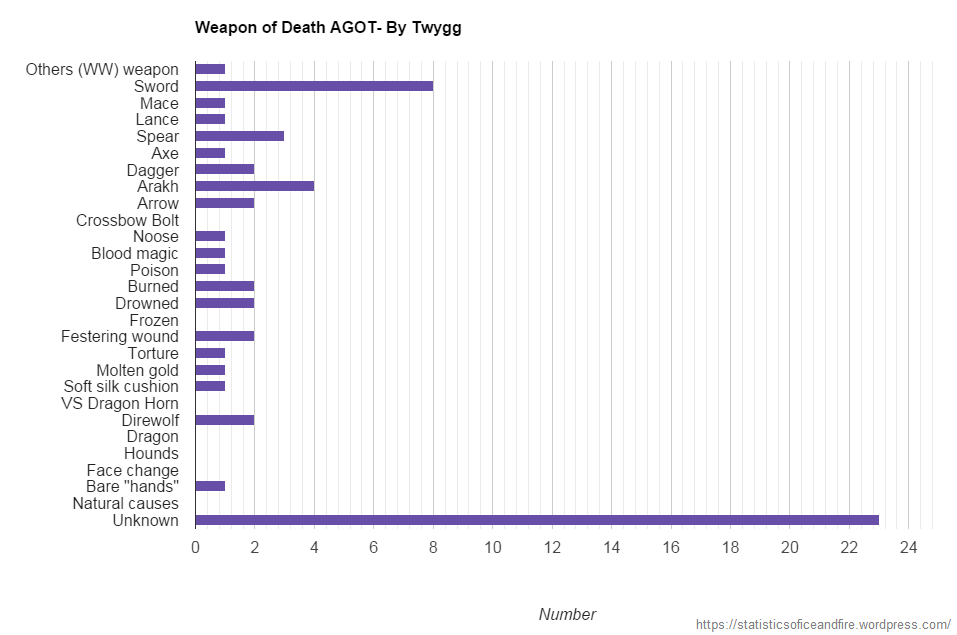
\includegraphics[width=0.9\linewidth]{weaponofdeath}
\end{figure}
\cite{p8}
\end{frame}

\begin{frame}
\begin{block}{}
Чем это плохо? 
\end{block}
Ничем. Это хорошо {\Large \Smiley{}}.\par
Но, кажется, таким образом мы~упускаем литературоведческую фактуру. Получается слишком \alert{distant} reading.
\begin{block}{}
При таком подходе
\end{block}
\begin{itemize}
\item на~месте <<Песни льда и~огня>> могла быть какая угодно книга;
\item данные часто (хотя и~не всегда) берутся не~из собственно текста, а~из энциклопедии вымышленного мира http://awoiaf.westeros.org/.
\end{itemize}
\end{frame}
%------------------------------------------------

\begin{frame} % Need to use the fragile option when verbatim is used in the slide
\frametitle{Признаки в алгоритмах машинного обучения}
\begin{example}[Feature list в \cite{p4}]
House to which a character belongs \par
Social group to which a character belongs \par
Male or female \par
Character's appearance in the book (все книги по отдельности)\par
Number of dead characters to whom a character is related \par
Whether the character is married \par
\dots
\end{example}

\centering \LARGE{Что не так с этим списком?}

\end{frame}

\begin{frame}
\frametitle{Что же не так?}
\begin{block}{}
Эти признаки не отражают \alert{поэтику} произведения.
\end{block}
Перечисленные признаки, разумеется, не~случайны. Они взяты из~практики применения анализа данных в~жизни. Для~\alert{человека} с~точки зрения статистики признаки принадлежности \textit{семье}, \textit{социальной группе}, \textit{пол}, \textit{состояние в~браке} "--- осмысленны.\par
Для~\alert{персонажа} это не~обязательно так.\par
Здесь мы~видим отражение отношений \alert{в вымышленном мире}, а~не~отражение поэтики. Из"=за этого исследователь, который подошел к~тексту с~таких позиций, выглядит как вульгарный социолог, потому что~не~видит текста и~не обращает внимание на~то, как он~построен.
\parskip=12pt
\par
\small{Конечно, устройство вымышленного мира тоже отражает поэтику, но~косвенно}

\end{frame}

\begin{frame}
\frametitle{Что же не так?}
\begin{block}{Положительный пример}
\cite{p6} За~основу своего исследования авторы работы взяли электронную версию книги «Буря мечей», так как, по~их словам, именно в~этой книге повествование достигло достаточного развития. В~качестве «связи» (фактически ребром графа) между персонажами выступало упоминание имен друг друга в~диапазоне 15 слов. Таким образом, связь героев друг с~другом вовсе не~означает, что~они друзья, "--- скорее, это просто говорит о~том, что~они взаимодействуют, говорят друг о~друге или~упоминаются вместе. В~результате, они получили граф, отражающий значимость персонажей.
\end{block}

Взаимодействие в~тексте "--- это уже поэтика.

\end{frame}

\begin{frame}
\begin{figure}
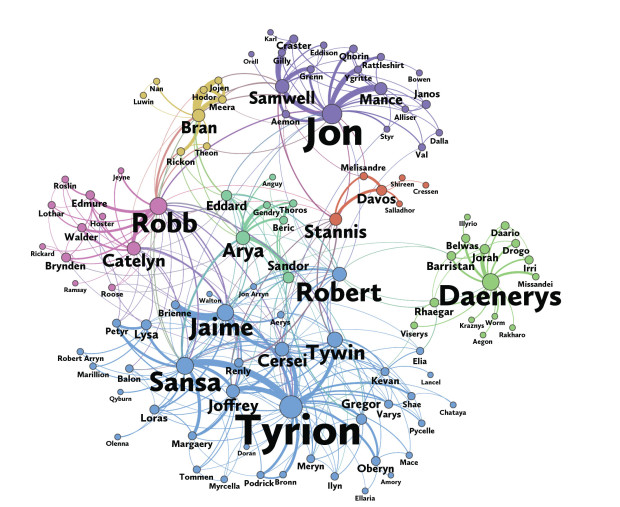
\includegraphics[width=0.8\linewidth]{networkofthrones}
\end{figure}
\cite{p6}
\end{frame}

\begin{frame}
Ср. другой социальный граф, отражающий диалоги персонажей:
\begin{figure}
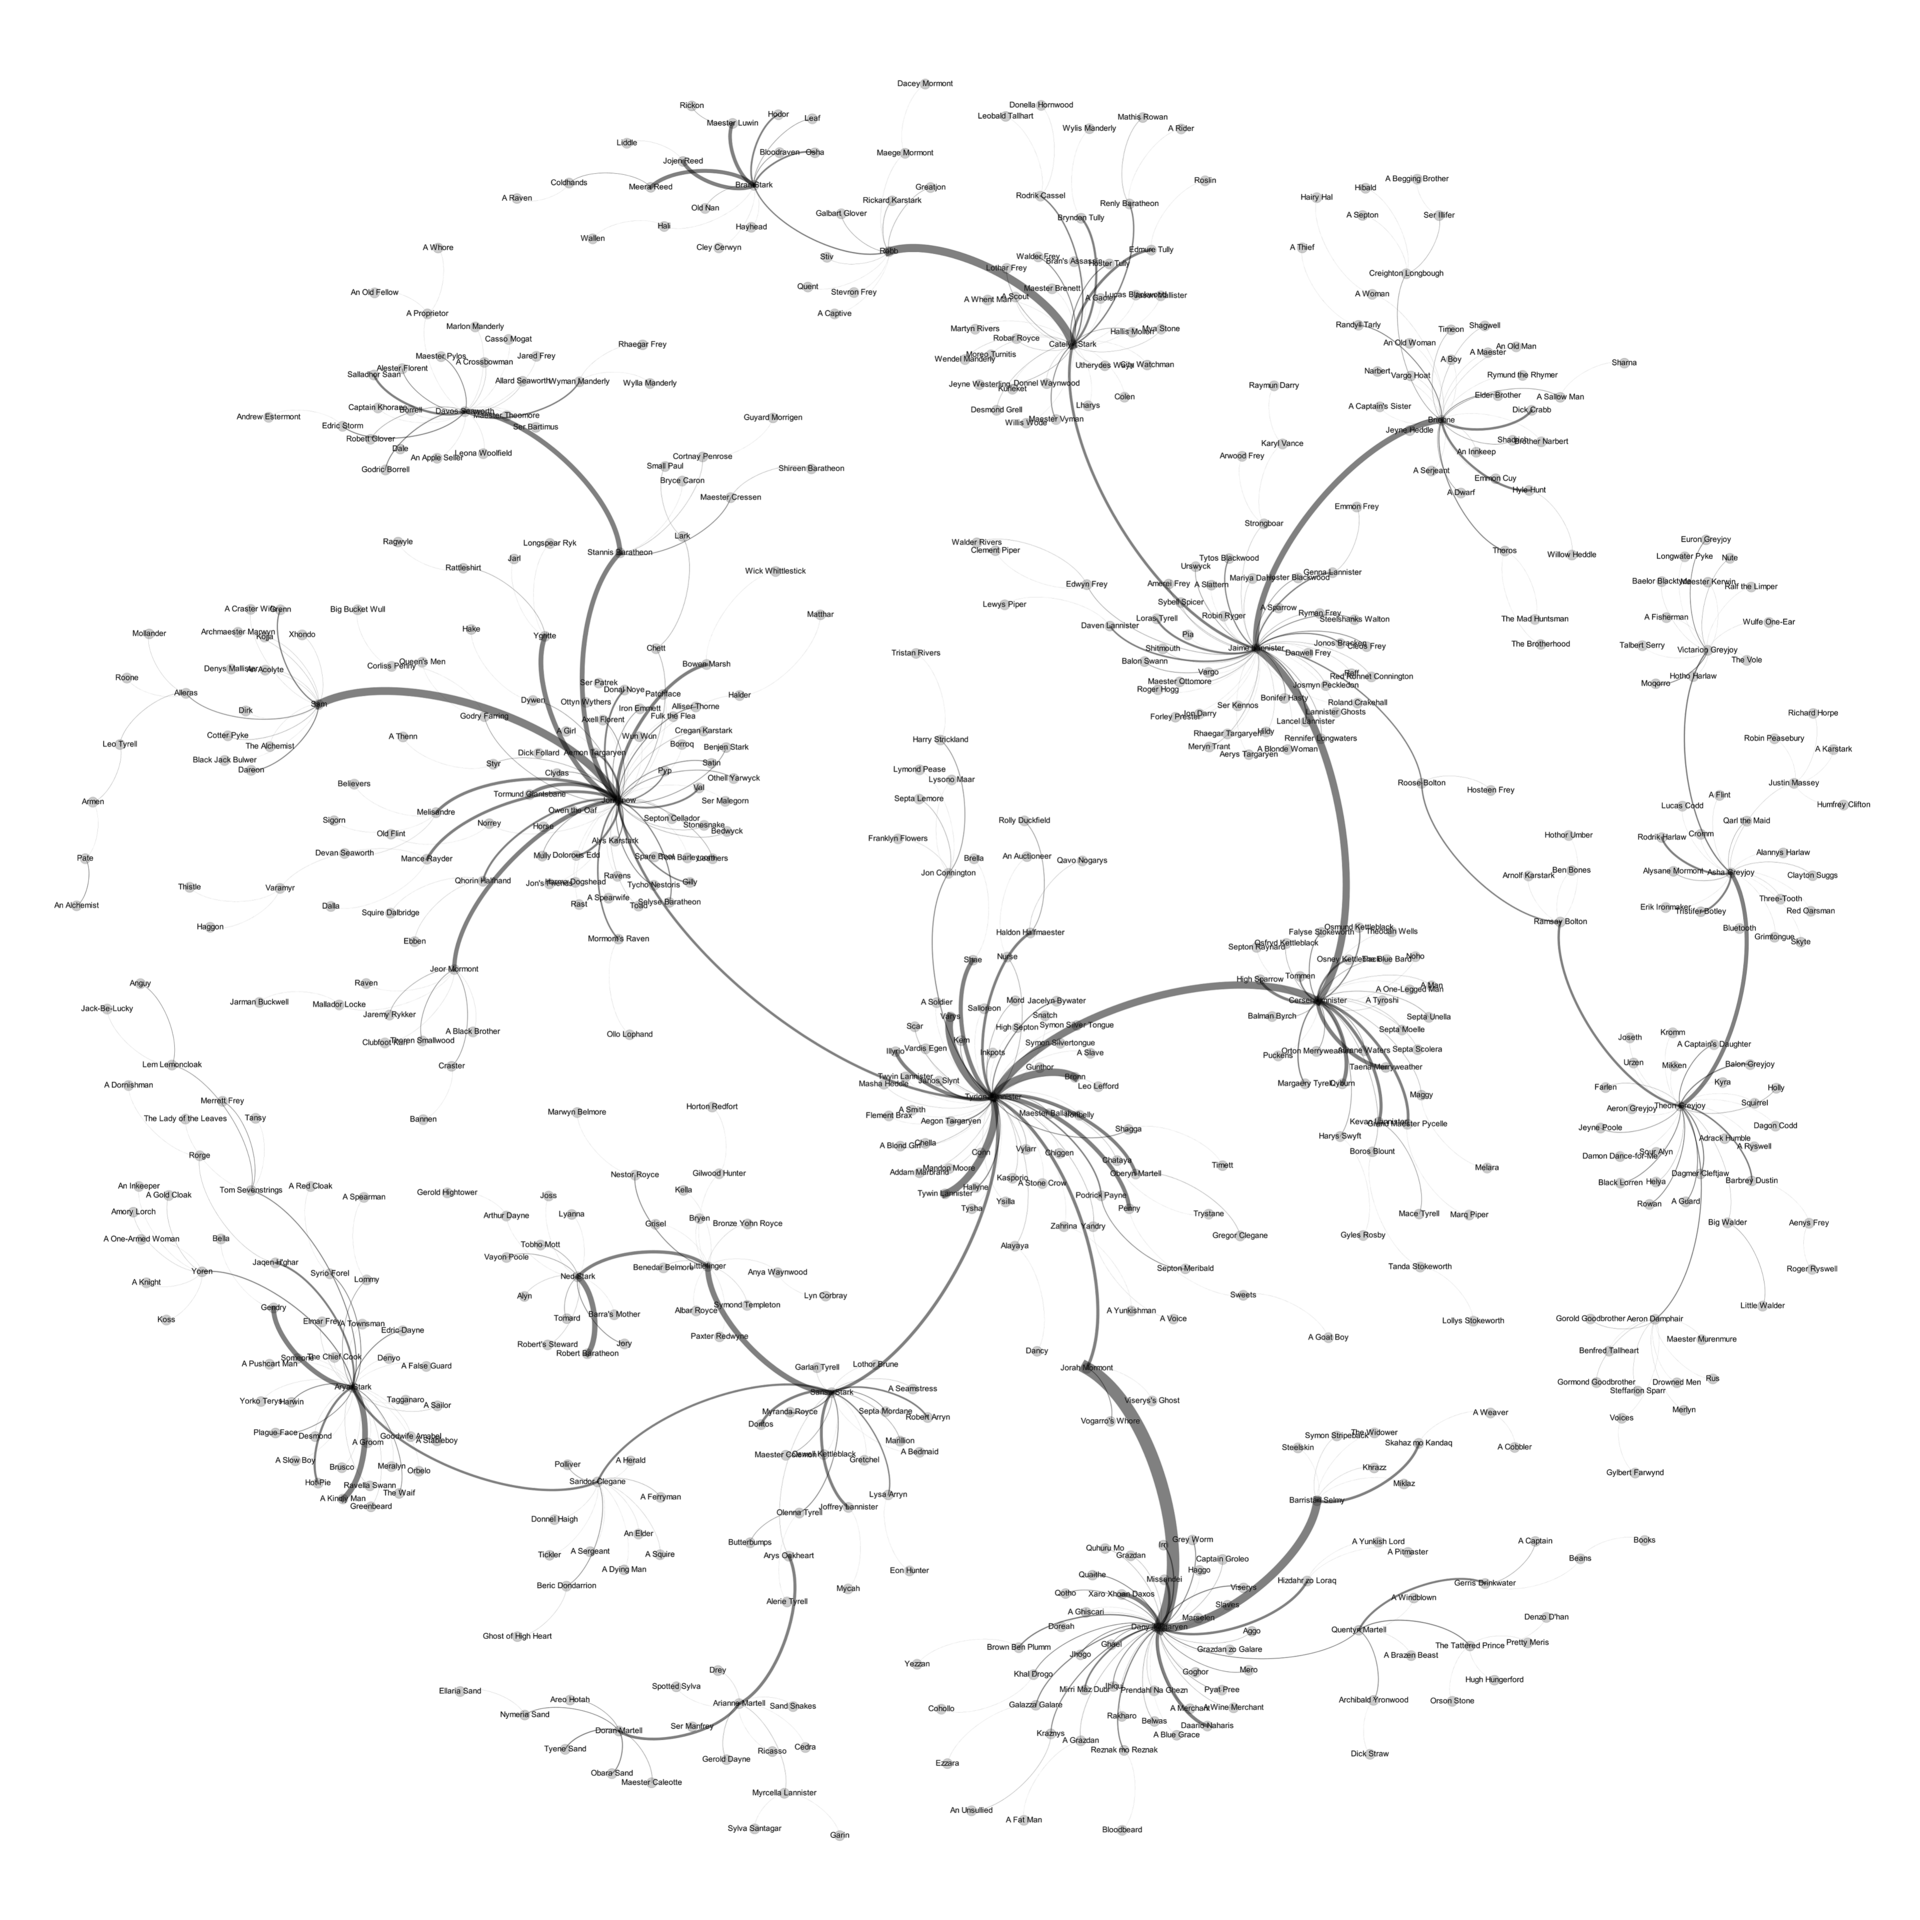
\includegraphics[width=0.6\linewidth]{networkofthrones2}
\end{figure}
\cite{p10}
\end{frame}

\subsection{Как встретиться литературоведению и анализу данных?}

\begin{frame}
\frametitle{Чем будем заниматься мы?}

\begin{block}{Литературоведение и анализ данных}
Основная задача нашей работы в~том, чтобы литературоведение и~анализ данных встретились, и~их объединение было \alert{не~механическим}. Мы~должны найти в~тексте такие параметры для~анализа, которые бы
\end{block}
\begin{enumerate}
\item соотносились с~поэтикой произведения (а~не~просто были~бы привычны для~аналитиков, использующих статистику), 
\item извлекались из~текста (а~не~из вторичных источников),
\item могли получить литературоведческую интерпретацию (почти то~же, что~первое, но~не~совсем)
\item были статистически верно обработаны (само собой)
\end{enumerate} 

\end{frame}

\section{Задачи, материал, методы}

\begin{frame}
\frametitle{Что будем считать мы?}
\begin{columns}[c] % The "c" option specifies centered vertical alignment while the "t" option is used for top vertical alignment

\column{.45\textwidth} % Left column and width
\textbf{Исследовательские сюжеты}
\begin{enumerate}
\item Цвета
\item Субъекты повествования
\item Персонажи
\item Топонимы
\end{enumerate}

\column{.5\textwidth} % Right column and width
Сначала определимся с~тем, что~эти направления анализа не~случайны и~информативны именно для~поэтики <<Песни льда и~пламени>>.

\end{columns}
\end{frame}

\begin{frame}
\frametitle{Цвета}

\begin{block}{Дж. Р. Р. Мартин в интервью:}
Фэнтези "--- серебро и~багрянец, индиго и~лазурь, обсидиан с~прожилками золота и~лазурита. А~реальность "--- это фанера и~пластик, окрашенные в~грязно"=коричневые и~желтовато"=зеленые тона. Фэнтези имеет вкус хабанеры и~меда, корицы и~гвоздики, превосходного красного мяса и~вина, сладкого, словно лето. Реальность "--- это бобы и~тофу, а~в~конечном итоге "--- прах.
\end{block}
\begin{itemize}
\item Цвета навязчиво встречаются в каждом описании: 
\begin{itemize}
\item Jon's eyes were a \alert{grey} so dark they seemed almost \alert{black} (GoT, Bran I)
\item She wore a garland of \alert{pale blue} roses, and her eyes wept blood (GoT, Eddard XIII)
\end{itemize}
\item Многие значимые имена и названия включают цвета: Серый Ветер, Чёрный замок.
\end{itemize} 

\end{frame}

%------------------------------------------------


\begin{frame}
\frametitle{Субъекты повествования (POV)}

\begin{itemize}
\item Важный конструктивный элемент текста.
\end{itemize} 

\begin{figure}
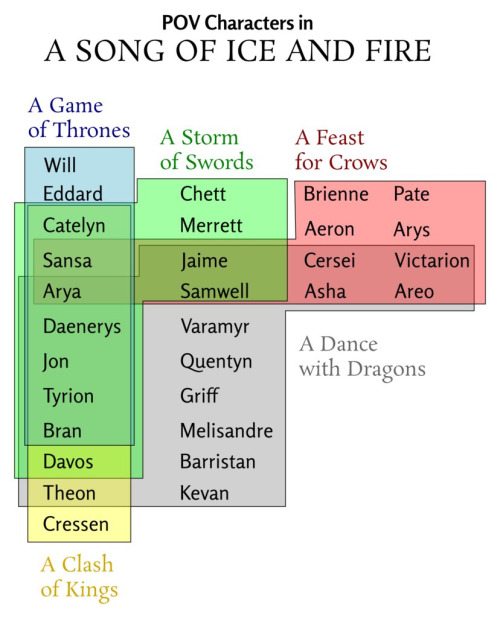
\includegraphics[width=0.5\linewidth]{POVs}
\end{figure}

\end{frame}

\begin{frame}
\frametitle{Перонажи}

\begin{itemize}
\item Важная составляющая поэтики нарративного текста.
\end{itemize} 

\begin{figure}
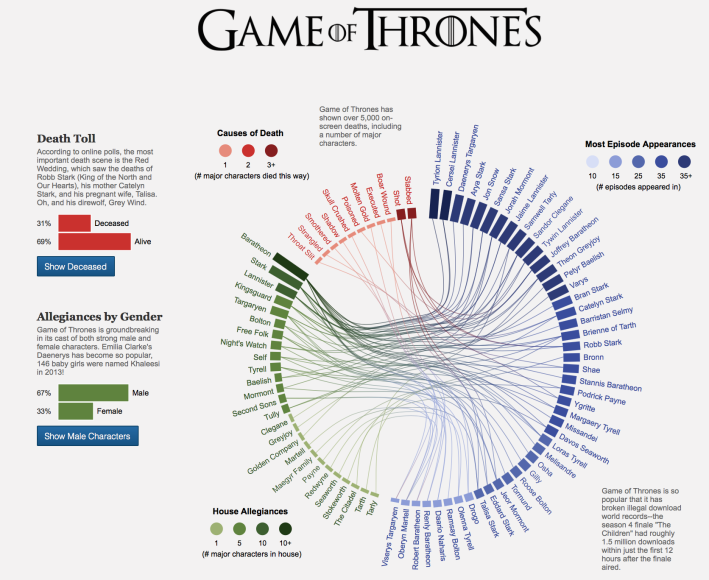
\includegraphics[width=0.5\linewidth]{got_heroes}
\end{figure}
http://thronesviz.github.io/
\end{frame}

\begin{frame}
\frametitle{География}

\begin{itemize}
\item Способ организации художественного пространства.
\item Правда ли это отличается от принадлежности дому, которую можно взять из энциклопедии?
\end{itemize} 

\begin{figure}
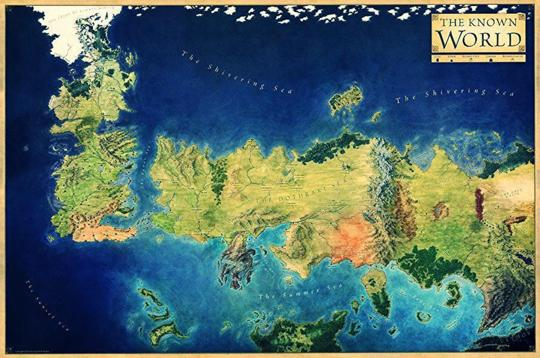
\includegraphics[width=0.5\linewidth]{Map}
\end{figure}
\end{frame}

\begin{frame}
\frametitle{Как?}

\begin{center}
	{\LARGE Компьютерная лингвистика и анализ данных!}
\end{center}

Репозиторий с кодом и данными: https://github.com/nevmenandr/Martin\_tutorial

\end{frame}

%------------------------------------------------

%------------------------------------------------

\begin{frame}
\begin{figure}
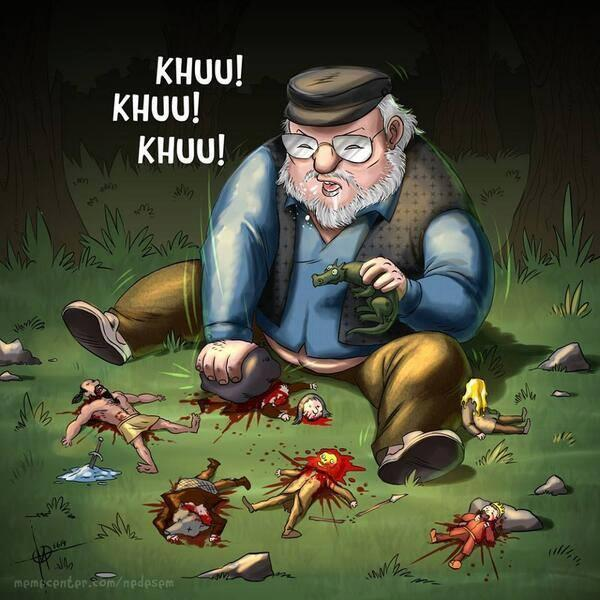
\includegraphics[width=0.7\linewidth]{grrm-beetles-}
\end{figure}
\end{frame}

%------------------------------------------------

\begin{frame}
\frametitle{Ссылки}
\footnotesize{
\begin{thebibliography}{99} % Beamer does not support BibTeX so references must be inserted manually as below
\bibitem[Guy Yachdav et al, 2016]{p1} Guy Yachdav et al (2016)
\newblock Song of Ice and Data
\newblock \emph{https://got.show/} 

\bibitem[Allen Downey, 2015]{p2} Allen Downey (2015)
\newblock Bayesian survival analysis for <<Game of Thrones>>
\newblock \emph{http://allendowney.blogspot.ru/2015/03/bayesian-survival-analysis-for-game-of.html} 

\bibitem[Éric Ledu, 2014]{p3} Éric Ledu (2014)
\newblock Data Geek III - Analyzing Games Of Thrones Data for the GoT Challenge
\newblock \emph{http://scn.sap.com/community/lumira/blog/2014/12/11/data-geek-iii--analyzing-games-of-thrones-data-for-the-got-challenge} 

\bibitem[Guy Yachdav et al, 2016a]{p4} Guy Yachdav et al (2016a)
\newblock How do we predict likelihood of death?
\newblock \emph{https://got.show/machine-learning-algorithm-predicts-death-game-of-thrones}

\bibitem[Maxime, 2016]{p5} Maxime (2016)
\newblock Summer is Coming - Game of Thrones Analytics
\newblock \emph{http://www.dataiku.com/blog/2016/04/23/got-analytics.html}

\end{thebibliography}
}
\end{frame}

\begin{frame}
\frametitle{Ссылки}
\footnotesize{
\begin{thebibliography}{99}

\bibitem[Andrew Beveridge and Jie Shan, 2016]{p6} Beveridge, Shan (2016)
\newblock Network of Thrones
\newblock \emph{Math Horizons} Vol. 23, No. 4 (April 2016), pp. 18-22

\bibitem[Unknown, 2015]{p7} Unknown (2015)
\newblock (Spoilers All) I made a word count of the whole ASOIAF books
\newblock \emph{https://www.reddit.com/r/asoiaf/comments/3froem/spoilers\_all\\\_i\_made\_a\_word\_count\_of\_the\_whole}

\bibitem[Ember Twygg, 2015]{p8} Ember Twygg (2015)
\newblock Statistics of Ice and Fire
\newblock \emph{https://statisticsoficeandfire.wordpress.com/} 

\bibitem[Азат Хузияхметов, 2016]{p9} Азат Хузияхметов (2016)
\newblock Игра Престолов в числах
\newblock \emph{https://geektimes.ru/post/275466/}

\bibitem[Азат Хузияхметов, 2016a]{p10} Азат Хузияхметов (2016a)
\newblock Теория графов в Игре Престолов
\newblock \emph{https://habrahabr.ru/post/302936/}

\end{thebibliography}
}
\end{frame}

\begin{frame}
\frametitle{Ссылки}
\footnotesize{
\begin{thebibliography}{99}

\bibitem[Erik Germani, 2016]{p11} Erik Germani (2016)
\newblock A Study of Ice and Fire
\newblock \emph{http://atseajournal.com/asoiaf/}



\end{thebibliography}
}
\end{frame}

%------------------------------------------------

\begin{frame}
\Huge{\centerline{That's all Folks!}}
\end{frame}

%----------------------------------------------------------------------------------------

\end{document}